\documentclass[]{article}


\usepackage[utf8]{inputenc}
\usepackage{hyperref}
\usepackage[acronym]{glossaries}
\usepackage{graphicx}

%--------------------packages fore vhdl stuff----------------------------
\usepackage[T1]{fontenc}
\usepackage{beramono}% monospaced font with bold variant

\usepackage{listings}
\lstdefinelanguage{VHDL}{
	morekeywords={
		library,use,all,entity,is,port,in,out,end,architecture,of,
		begin,and
	},
	morecomment=[l]--
}

\usepackage{xcolor}
\colorlet{keyword}{blue!100!black!80}
\colorlet{comment}{green!90!black!90}
\lstdefinestyle{vhdl}{
	language     = VHDL,
	basicstyle   = \ttfamily,
	keywordstyle = \color{keyword}\bfseries,
	commentstyle = \color{comment}
}

%--------------------todo stuff-----------------------------------------
\usepackage[colorinlistoftodos,prependcaption,textsize=tiny]{todonotes}
%opening
\hypersetup{
	colorlinks,
	citecolor=black,
	filecolor=black,
	linkcolor=black,
	urlcolor=black
}

%---------------------hyper link stuff------------------------------------
\usepackage{hyperref}
\hypersetup{
	colorlinks,
	citecolor=black,
	filecolor=black,
	linkcolor=black,
	urlcolor=black
}

%opening
%-----------------------glossary-------------------------------------------
\makenoidxglossaries % use TeX to sort

%
\loadglsentries{glos_list.tex}
\title{Technical status Zifra card}
\author{Torbjörn}

\begin{document}

\maketitle
\tableofcontents
\newpage
\newpage

\begin{abstract}
This document will summarize have bin done and what is needed to do to get to the final product.
\end{abstract}

\newpage


\section{todo}
Here i will list stuff i come up whit so that i can write about them later.

\begin{itemize}
	\item crypto scheem whit curv 25519
	\item Alex algorithm
	\item hiding files in fat
	\item fat format
\end{itemize}

\section{Brief description}
We will here shortly describe what the Zifra card is meant to be.
It is an memory card that is supost to protect data by encrypting the data that is writen to it.
This is done whit the help of multiple \gls{keys} and \gls{cipher}.
i
\section{System overview}
We will here describe the way we want the system to work.
Fore the case of explenation we will use an camera as example case.
We will first talk about the key generation secondly encryption and finally about decryption step.

\subsection{Key generation}
There is three type of keys used in the crypto scheme.
The first two keys are pre-generated as an key pair on an safe device one \acrfull{priKey} and one \acrfull{pubKey}. 
The pri\_key is saved fore later use and the pub\_key is transfered and saved on the sd-card see Figure \ref{fig:key_gen}.
Then the user puts the sd card in an camera.
When the camera boots up an random number is generated this is the \acrfull{randKey} this number is then encrypted whit the Pub\_key and saved on the memory.

\begin{figure}[h]
	\centering
	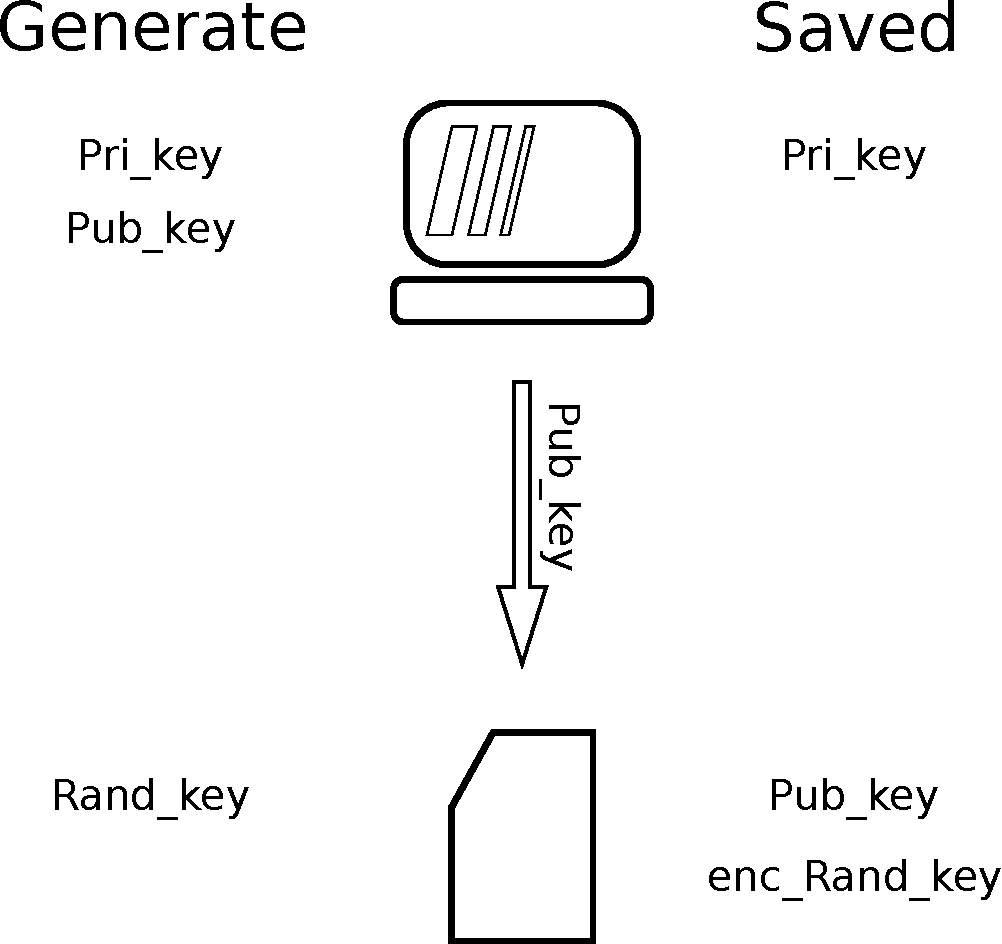
\includegraphics[width=0.8\textwidth]{ilustrations/Key_generations.pdf}
	\caption{This illustration shows where the keys are generated and where they are stored}
	\label{fig:key_gen}
\end{figure}
\clearpage
\newpage
\subsection{Encryption}
The Rand\_key\footnote{This is the non encrypted random key.} is then used as the key input in the chacha cipher to encrypt the data before it is saved to the memory se Figure \ref{fig:encrypt}.
When the system is powered of the Rand\_key that is only stored in the FPGA disappeared due to the nature of an FPGA.
The generation and encryption of the Rand\_key is repeated fore each session.
So there will be multiple enc\_Rand\_key:s stored on the memory one fore each session.

\begin{figure}[h]
	\centering
	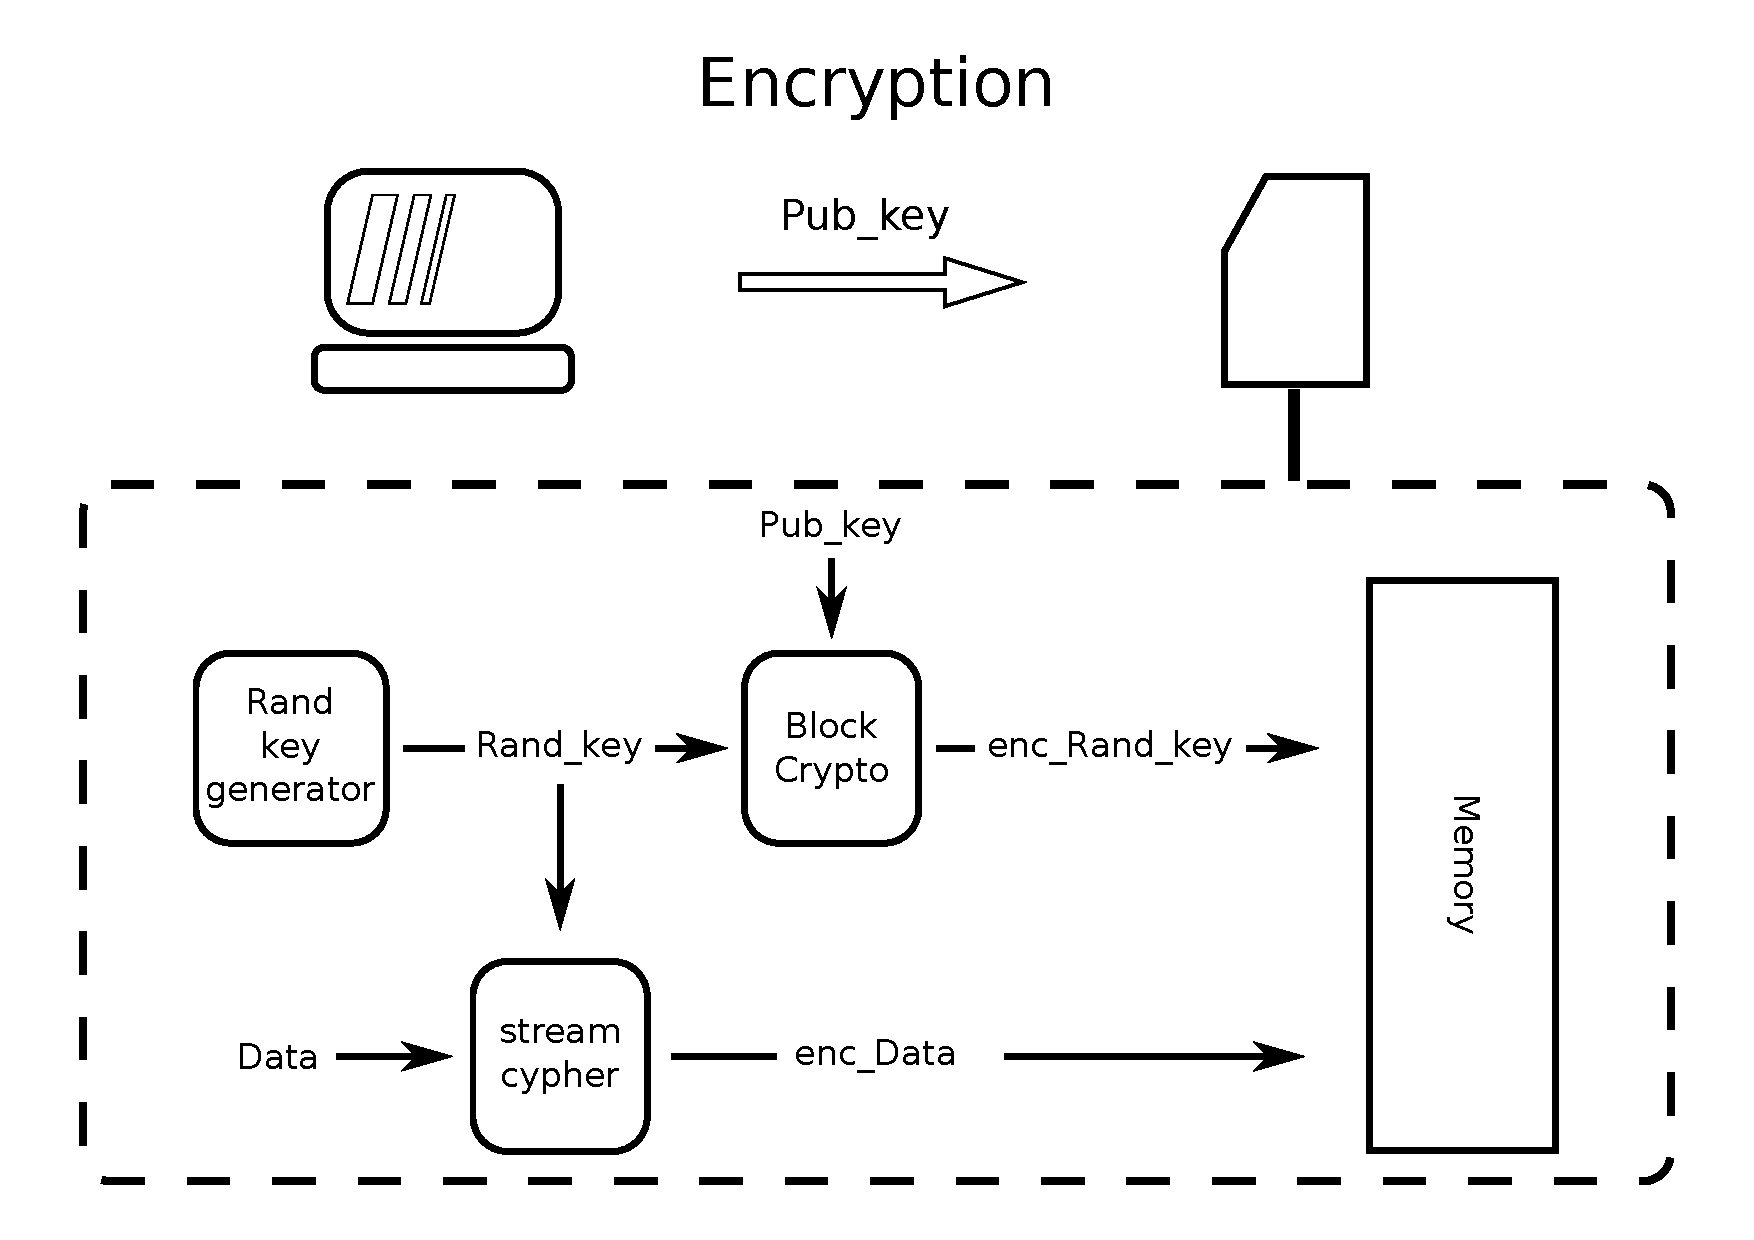
\includegraphics[width=0.8\textwidth]{ilustrations/encryption.pdf}
	\caption{Basic data flow in encryption step}
	\label{fig:encrypt}
\end{figure}
\clearpage
\newpage
\subsection{Decryption}
When decrypting the data one extracts the encrypted data and the \acrfull{encRandKey} on to the safe device were the Pri\_key is saved.
Then we use the Pri\_key to decrypt the enc\_Rand\_key:s and then we can use the Rand\_key:s to decrypt the data se Figure \ref{fig:decrypt}.

\begin{figure}[h]
	\centering
	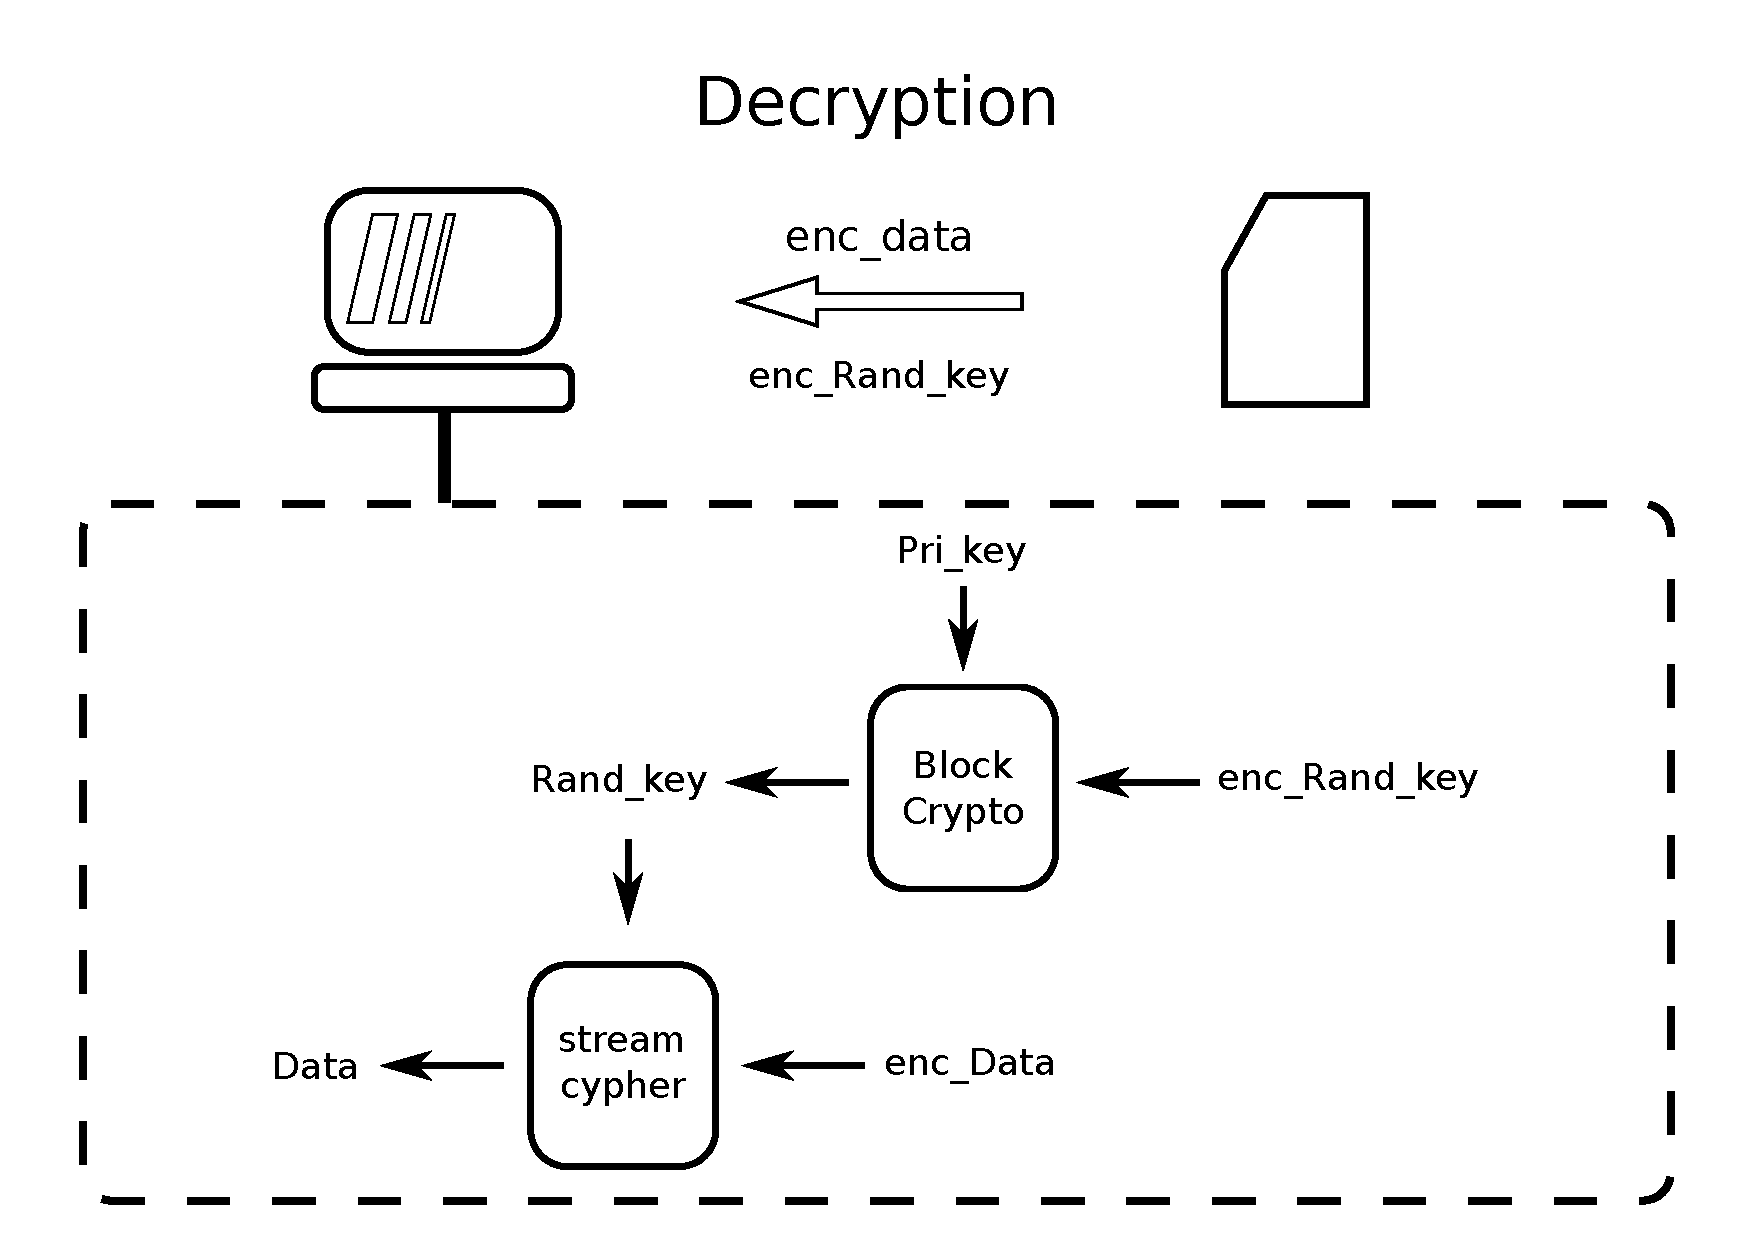
\includegraphics[width=0.8\textwidth]{ilustrations/decryption.pdf}
	\caption{basic data flow in decryption step}
	\label{fig:decrypt}
\end{figure}



\section{Hardware}
The hardware was intended to be an \acrfull{pcb} whit an \acrfull{fpga} whit an memory and some suport component.
The FPGA that we use is the Artix7 t35.


\section{sd slave progress}
The sd slave comes form the Google vault project \cite{GV}.
This part of the project dose not work yet.

We have extracted the blocks that we think are needed fore the project.
There test bench to test and send commands to the design and see what responses the device sends back.
So fare we can read and write from the first sector in the memory but not to any other once \todo{need to bouble check this whit mesages from antti.}. 

\section{chacha}
The stream cipher that was decided to use fore the data encryption ip called chacha \cite{chacha} developed by Joachim Strömbergson \cite{joachim}.  
We have made an axi ip block out of it one stream port fore the data and one address port fore the setting of iv and key \todo{Probebly more ports here look in the design.}
There is also an test case whit an micro blaze and an firmware to demonstrate how the axi crypto works.  


\section{Helpful data}
This section will list information that have bin collected during the project that might help further development.

\subsection{CSD list}
During the debugging we listed the CSD values that was used in the \gls{gvsdslave} we also made an list of the other CSD values.

\section{Whishlist}
Here we will list some features that we wold like to have in the future.
Thees are extras but good to have.

\subsection{Hidden files}
We wold like to have the possibility to hide the files so that every time you start up the memory card it looks empty.
This wold be don by making an temporary FAT table that is used during the session then hidden between the \gls{mbs} and the real FAT table.

\subsection{See pictures when camera is still on}
We wold like to be able to look at the pictures during the session.
This wold mean that the cipher needs to work in both directions during the session.

\subsection{Fake pictures}
We wold also like to be able to prep the memory card whit fake data in the camera case that wold be preloaded whit pictures.
Thees wold show up if someone wold inspect the card.
This wold also be helped by the see pictures while session is active if the system is tested.

\todo{add the CSD tables here}


\clearpage
\newpage
\printglossary[type=\acronymtype]
\printnoidxglossaries


\bibliography{mybib}{}
\bibliographystyle{plain}
\end{document}

 












